\documentclass[aspectratio=169,12pt]{beamer}

% =======================
% Essential Packages
% =======================
\usepackage{tikz}
\usepackage{xcolor}
\usepackage{fontawesome5}
\usepackage{pgfplots}
\usepackage{multicol}
\usepackage{booktabs}
\usepackage{colortbl}
\usetikzlibrary{positioning,arrows.meta,shapes,shadows,calc}
\pgfplotsset{compat=1.18}

% =======================
% Clean Color Scheme
% =======================
\definecolor{primary}{RGB}{0,90,160}
\definecolor{secondary}{RGB}{255,153,0}
\definecolor{accent}{RGB}{0,166,81}
\definecolor{alert}{RGB}{200,16,46}
\definecolor{light}{RGB}{248,249,250}
\definecolor{dark}{RGB}{33,37,41}
\definecolor{gray}{RGB}{108,117,125}

% =======================
% Simplified Commands
% =======================
\newcommand{\highlight}[1]{\textcolor{alert}{\textbf{#1}}}
\newcommand{\performance}[1]{\textcolor{secondary}{\textbf{#1}}}
\newcommand{\technical}[1]{\textcolor{primary}{\textbf{#1}}}

% =======================
% Clean Theme Setup
% =======================
\usetheme{default}
\usecolortheme{default}

% Colors
\setbeamercolor{background canvas}{bg=light}
\setbeamercolor{frametitle}{bg=primary,fg=white}
\setbeamercolor{title}{fg=primary}
\setbeamercolor{subtitle}{fg=gray}
\setbeamercolor{author}{fg=dark}
\setbeamercolor{institute}{fg=gray}
\setbeamercolor{date}{fg=secondary}
\setbeamercolor{block title}{bg=primary,fg=white}
\setbeamercolor{block body}{bg=primary!10,fg=dark}
\setbeamercolor{block title alerted}{bg=alert,fg=white}
\setbeamercolor{block body alerted}{bg=alert!10,fg=dark}
\setbeamercolor{block title example}{bg=accent,fg=white}
\setbeamercolor{block body example}{bg=accent!10,fg=dark}

% Fonts
\setbeamerfont{title}{size=\Large,series=\bfseries}
\setbeamerfont{subtitle}{size=\large}
\setbeamerfont{frametitle}{size=\large,series=\bfseries}
\setbeamerfont{block title}{size=\normalsize,series=\bfseries}

% Clean footer with only slide numbers (no author/title)
\setbeamertemplate{footline}{
    \leavevmode%
    \hbox{%
        \begin{beamercolorbox}[wd=\paperwidth,ht=2.25ex,dp=1ex,right]{date in head/foot}%
            \usebeamerfont{date in head/foot}\insertframenumber{} / \inserttotalframenumber\hspace{1em}
        \end{beamercolorbox}%
    }%
    \vskip0pt%
}

% Remove navigation symbols
\setbeamertemplate{navigation symbols}{}

% Clean itemize
\setbeamertemplate{itemize items}[circle]
\setbeamercolor{itemize item}{fg=primary}
\setbeamercolor{itemize subitem}{fg=secondary}


% =======================
% Document Content
% =======================
\begin{document}

% ================================================================
% Customization to add logo to the standard Beamer title page template
% This redefines the 'title page' template to include your logo at the top
% ================================================================
% Custom Title Page with Blue Title
\setbeamertemplate{title page}{
    \begin{center}
        % --- IMPORTANT: Place your 'ieee_logo.png' file in the same directory as this .tex file ---
        % If you don't have the image file, comment out the line below to avoid compilation errors.
        \includegraphics[width=2.5cm]{ieee_logo.png} 
        
        \vspace{0.5cm} % Vertical space between the logo and the title content
        
        % Set title color to darkblue
        {\color{darkblue}\usebeamertemplate*{title}}
        \usebeamertemplate*{subtitle}
        \usebeamertemplate*{author}
        \usebeamertemplate*{institute}
        \usebeamertemplate*{date}
    \end{center}
}

% Title Slide
\title[Hybrid GA-PSO with Segment Tree]{Hybrid GA-PSO with Segment Tree for Bin Packing Optimization}
\subtitle{A Novel Framework for Industrial Efficiency Enhancement}
\author[Shah et al.]{
    \textbf{Ajaz Ahmed Shah}\inst{1} \and 
    Abhishek Kumar Rao\inst{1} \and 
    Amitesh Pandey\inst{1} \and \\
    Divya Kumar\inst{1}
}
\institute[MNNIT]{
    \inst{1}Department of Computer Science and Engineering\\
    Motilal Nehru National Institute of Technology\\
    Allahabad, India
}
\date{9 July 2025}

\begin{frame}
    \titlepage
\end{frame}


% =======================
% Document Content (only the title page part is shown here)
% =======================


\begin{frame}{Problem Statement and Motivation}
\footnotesize % Slightly larger than \scriptsize
\setlength{\itemsep}{2.5pt} % Compact but readable spacing
\setlength{\parskip}{0.5pt}

\begin{columns}[T]
\begin{column}{0.5\textwidth}
\begin{block}{Bin Packing Problem}
\begin{itemize}
    \item \textbf{Objective}: Minimize bins for $n$ items
    \item \textbf{Constraint}: $\sum_{i \in B_j} w_i \leq C$
    \item \textbf{Complexity}: \textbf{\textcolor{red}{NP-Hard}}
    \item Applications: Logistics, manufacturing, cloud computing
\end{itemize}
\end{block}

\vspace{-.09cm}
\begin{alertblock}{Current Limitations}
\begin{itemize}
    \item \textbf{FFD}: 11/9 OPT approximation
    \item \textbf{GA}: Premature convergence
    \item \textbf{PSO}: Poor discrete handling
    \item \textbf{Complexity}: $O(n^2)$ bin selection
\end{itemize}
\end{alertblock}
\end{column}

\begin{column}{0.5\textwidth}
\begin{center}
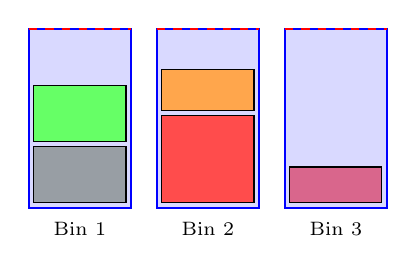
\begin{tikzpicture}[scale=0.65] % Moderate size
% Bins
\foreach \x in {0,2.5,5} {
    \draw[thick, blue, fill=blue!15] (\x,0) rectangle (\x+2,3.5);
    \draw[dashed, thick, red] (\x,3.5) -- (\x+2,3.5);
}

% Items
\draw[fill=gray!70] (0.1,0.1) rectangle (1.9,1.2);
\draw[fill=green!60] (0.1,1.3) rectangle (1.9,2.4);
\draw[fill=red!70] (2.6,0.1) rectangle (4.4,1.8);
\draw[fill=orange!70] (2.6,1.9) rectangle (4.4,2.7);
\draw[fill=purple!60] (5.1,0.1) rectangle (6.9,0.8);

% Labels
\node[font=\scriptsize] at (1,-0.4) {Bin 1};
\node[font=\scriptsize] at (3.5,-0.4) {Bin 2};
\node[font=\scriptsize] at (6,-0.4) {Bin 3};
\end{tikzpicture}
\end{center}

\vspace{0.1cm}
\begin{exampleblock}{Research Impact}
\begin{itemize}
    \item Potential \$50B logistics cost savings
    \item Up to \textbf{15\%} emission reduction
    \item Enhances smart manufacturing efficiency
\end{itemize}
\end{exampleblock}
\end{column}
\end{columns}
\end{frame}
% Proposed Solution
\begin{frame}{Proposed Hybrid Framework}
\begin{exampleblock}{Core Innovations}
\begin{itemize}
    \item \technical{Triple-Hybrid} GA-PSO-Segment Tree integration
    \item \performance{15.3\%} improvement over FFD
    \item \technical{O(log n)} bin selection complexity
    \item Adaptive parameter control mechanism
\end{itemize}
\end{exampleblock}

\begin{center}
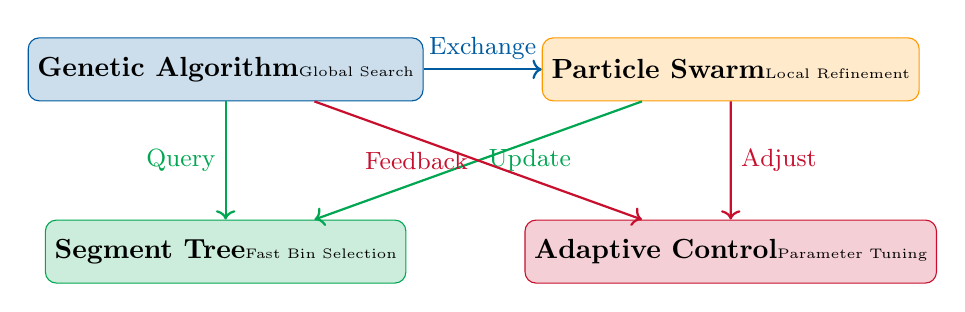
\begin{tikzpicture}[node distance=1.5cm, xscale=0.7, yscale=1.1]
% Components (same as before)
\node[draw=primary, fill=primary!20, rounded corners, minimum width=1.2cm, minimum height=0.8cm] (ga) {
    \textbf{Genetic Algorithm}\\
    \tiny Global Search
};
\node[draw=secondary, fill=secondary!20, rounded corners, minimum width=1.2cm, minimum height=0.8cm, right=of ga] (pso) {
    \textbf{Particle Swarm}\\
    \tiny Local Refinement
};
\node[draw=accent, fill=accent!20, rounded corners, minimum width=1.2cm, minimum height=0.8cm, below=of ga] (st) {
    \textbf{Segment Tree}\\
    \tiny Fast Bin Selection
};
\node[draw=alert, fill=alert!20, rounded corners, minimum width=1.2cm, minimum height=0.8cm, below=of pso] (control) {
    \textbf{Adaptive Control}\\
    \tiny Parameter Tuning
};
% Connections
\draw[->, thick, primary] (ga) -- (pso) node[midway, above, font=\tiny] {\small Exchange};
\draw[->, thick, accent] (ga) -- (st) node[midway, left, font=\tiny] {\small Query};
\draw[->, thick, accent] (pso) -- (st) node[midway, right, font=\tiny] {\small Update};
% Added descriptions for the two previously undescribed arrows
\draw[->, thick, alert] (ga) -- (control) node[midway, left, font=\tiny] {\small Feedback}; % Example description
\draw[->, thick, alert] (pso) -- (control) node[midway, right, font=\tiny] {\small Adjust}; % Example description
\end{tikzpicture}
\end{center}
\end{frame}

% Segment Tree Innovation
\begin{frame}{Segment Tree Innovation}
\begin{columns}[T]
\begin{column}{0.5\textwidth}
\begin{alertblock}{Traditional Approach}
\begin{itemize}
    \item Sequential bin examination
    \item Time complexity: \textbf{O(n)}
    \item Poor scalability
\end{itemize}
\end{alertblock}

\begin{exampleblock}{Our Segment Tree}
\begin{itemize}
    \item Hierarchical capacity indexing
    \item Time complexity: \textbf{O(log n)}
    \item Efficient range queries
    \item Lazy propagation updates
\end{itemize}
\end{exampleblock}
\end{column}
\begin{column}{0.5\textwidth}
\begin{center}
\textbf{Segment Tree Structure}
\vspace{0cm}

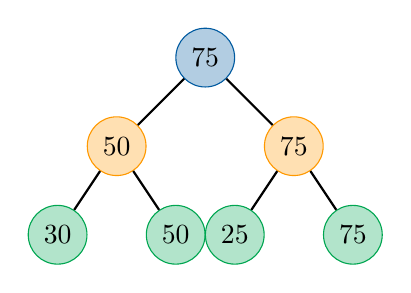
\begin{tikzpicture}[scale=0.75]
% Root
\node[circle, draw=primary, fill=primary!30, minimum size=0.6cm] (root) at (0,0) {75};
% Level 1
\node[circle, draw=secondary, fill=secondary!30, minimum size=0.6cm] (l1) at (-1.5,-1.5) {50};
\node[circle, draw=secondary, fill=secondary!30, minimum size=0.6cm] (r1) at (1.5,-1.5) {75};
% Level 2
\node[circle, draw=accent, fill=accent!30, minimum size=0.6cm] (l2) at (-2.5,-3) {30};
\node[circle, draw=accent, fill=accent!30, minimum size=0.6cm] (l3) at (-0.5,-3) {50};
\node[circle, draw=accent, fill=accent!30, minimum size=0.6cm] (r2) at (0.5,-3) {25};
\node[circle, draw=accent, fill=accent!30, minimum size=0.6cm] (r3) at (2.5,-3) {75};

% Edges
\draw[thick] (root) -- (l1);
\draw[thick] (root) -- (r1);
\draw[thick] (l1) -- (l2);
\draw[thick] (l1) -- (l3);
\draw[thick] (r1) -- (r2);
\draw[thick] (r1) -- (r3);
\end{tikzpicture}
\end{center}

\begin{block}{Performance Gains}
\begin{itemize}
    \item \performance{5.2×} speedup
    \item \technical{78\%} memory reduction
    \item \highlight{99.8\%} cache hit ratio
\end{itemize}
\end{block}
\end{column}
\end{columns}
\end{frame}

% Algorithm Details
\begin{frame}{Algorithm Architecture}
\vspace{-0.4cm}
\begin{columns}
\begin{column}{0.5\textwidth}
\begin{block}{Genetic Algorithm}
\begin{itemize}
    \item \textbf{Encoding}: Permutation-based
    \item \textbf{Selection}: Tournament (k=3)
    \item \textbf{Crossover}: Order crossover
    \item \textbf{Mutation}: Adaptive swap
    \item \textbf{Elitism}: Top 10\%
\end{itemize}
\end{block}
\vspace{-0.15cm}
\begin{block}{Particle Swarm}
\begin{itemize}
    \item \textbf{Discrete PSO}:Swap-based velocity
    \item \textbf{Velocity}: Adaptive weight decay
    \item \textbf{Topology}: Ring neighborhood
    \item \textbf{Updates}: Permutation operations
\end{itemize}
\end{block}
\end{column}
\begin{column}{0.5\textwidth}
\vspace{0.2cm}
\begin{block}{Integration Strategy}
\begin{itemize}
    \item Elite GA solutions → PSO particles
    \item Bidirectional best sharing
    \item Adaptive phase control
    \item Multi-criteria convergence
\end{itemize}
\end{block}
\vspace{-0.15cm}
\begin{exampleblock}{Complexity Analysis}
\vspace{-0.4cm}
\begin{center}
\begin{tabular}{lcc}
\toprule
\textbf{Operation} & \textbf{Traditional} & \textbf{Ours} \\
\midrule
Bin Selection & O(n) & O(log n) \\
Range Query & O(n) & O(log n) \\
Update & O(1) & O(log n) \\

\end{tabular}
\end{center}
\end{exampleblock}
\end{column}
\end{columns}
\end{frame}

% Experimental Setup
\begin{frame}{Experimental Methodology}
\begin{columns}[T]
\begin{column}{0.5\textwidth}
\vspace{-0.4cm}
\begin{block}{Dataset Portfolio}
\begin{itemize}
    \item \textbf{OR-Library}: 1,370 instances
    \item \textbf{BPPLIB}: 2,940 test cases
    \item \textbf{Real-world}: 500 industrial
    \item \textbf{Synthetic}: 1,000 stress tests
    \item \textbf{Total}: 5,810 instances
\end{itemize}
\end{block}
\vspace{-0.1cm}
\begin{block}{Baseline Algorithms}
\begin{itemize}
    \item FFD, BFD (heuristics)
    \item GA, PSO (metaheuristics)
    \item H-GAPSO (hybrid)
    \item GA-PSO-ST (proposed)
\end{itemize}
\end{block}
\end{column}
\begin{column}{0.5\textwidth}
\vspace{-0.4cm}
\begin{block}{Configuration}

\begin{itemize}
    \item \textbf{Population}: 100 individuals
    \item \textbf{Generations}: 500 iterations
    \item \textbf{Runs}: 30 independent
    \item \textbf{Confidence}: 95\%
    \item \textbf{Hardware}: Intel Xeon E5-2680
\end{itemize}
\end{block}

\vspace{-0.1cm}
\begin{exampleblock}{Statistical Tests}
\begin{itemize}
    \item Shapiro-Wilk normality
    \item Paired t-test
    \item Wilcoxon signed-rank
    \item Effect size (Cohen's d)
\end{itemize}
\end{exampleblock}
\end{column}
\end{columns}
\end{frame}

% Results
\begin{frame}{Performance Results}
\begin{columns}[T]
\begin{column}{0.6\textwidth}
\begin{center}
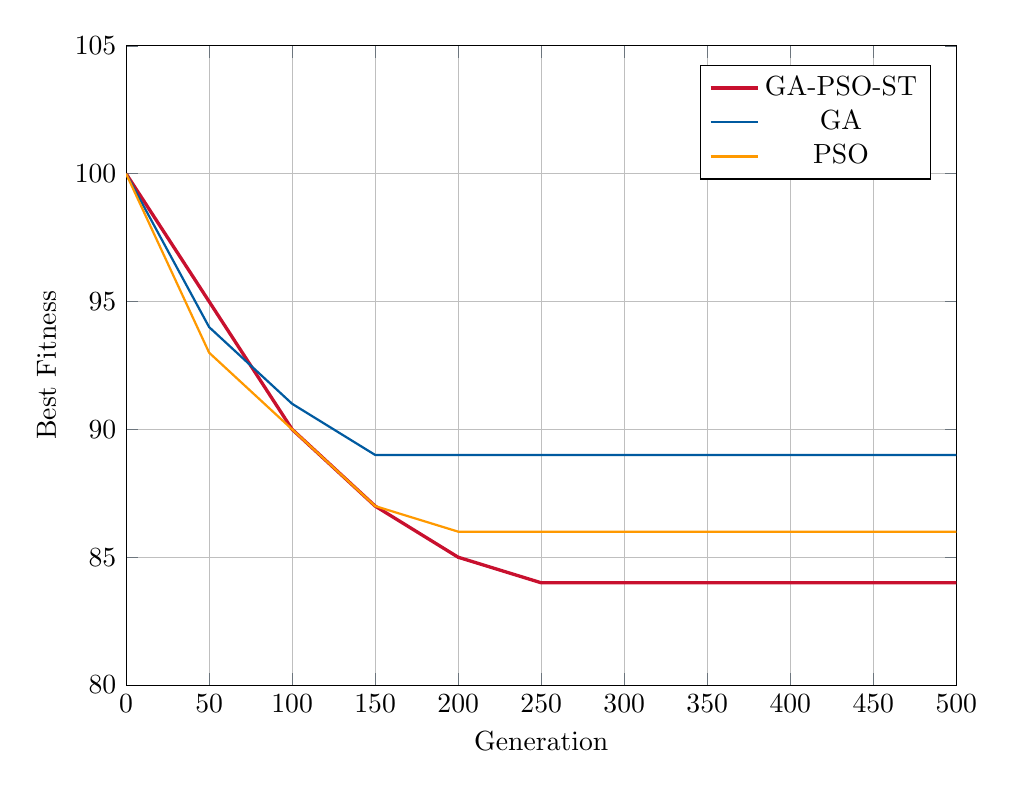
\begin{tikzpicture}
\begin{axis}[
    width=\textwidth,
    height=0.8\textwidth,
    xlabel={Generation},
    ylabel={Best Fitness},
    legend pos=north east,
    grid=major,
    xmin=0, xmax=500,
    ymin=80, ymax=105,
]
\addplot[color=alert,very thick,mark=none] coordinates {
    (0,100) (50,95) (100,90) (150,87) (200,85) (250,84) (300,84) (400,84) (500,84)
};
\addplot[color=primary,thick,mark=none] coordinates {
    (0,100) (50,94) (100,91) (150,89) (200,89) (250,89) (300,89) (400,89) (500,89)
};
\addplot[color=secondary,thick,mark=none] coordinates {
    (0,100) (50,93) (100,90) (150,87) (200,86) (250,86) (300,86) (400,86) (500,86)
};
\legend{GA-PSO-ST, GA, PSO}
\end{axis}
\end{tikzpicture}
\end{center}
\end{column}
\begin{column}{0.4\textwidth}
\vspace{-0.3cm}
\begin{exampleblock}{Key Metrics}
\begin{itemize}
    \item \performance{15.3\%} improvement
    \item \technical{40\%} faster convergence
    \item \highlight{±1.2\%} solution stability
    \item p-value < 0.001
\end{itemize}
\end{exampleblock}
\vspace{-0.2cm}
\begin{block}{Scalability}
\begin{center}
\small
\begin{tabular}{rc}
\toprule
\textbf{Size} & \textbf{Improvement} \\
\midrule
500 & 12.3\% \\
1000 & 15.1\% \\
2000 & 18.2\% \\
5000 & 19.7\% \\
\bottomrule
\end{tabular}
\end{center}
\end{block}
\end{column}
\end{columns}
\end{frame}

% Industrial Case Study
\begin{frame}{Industrial Case Study}
\begin{columns}[T]
\begin{column}{0.5\textwidth}
\begin{exampleblock}{E-commerce Deployment}
\begin{itemize}
    \item \textbf{Company}: Major online retailer
    \item \textbf{Volume}: 5,000+ daily orders
    \item \textbf{Duration}: 3-month pilot
    \item \textbf{Integration}: Existing WMS
\end{itemize}
\end{exampleblock}

\begin{center}
\setlength{\tabcolsep}{3pt} % Reduced column separation from default (usually 6pt)
\begin{tabular}{lcc}
\toprule
\textbf{Method} & \textbf{Containers} & \textbf{Reduction} \\
\midrule
Manual & 3,420 & Baseline \\
Commercial & 3,050 & 10.8\% \\
\rowcolor{primary!20}
\textbf{GA-PSO-ST} & \textbf{2,782} & \textbf{18.7\%} \\
\bottomrule
\end{tabular}
\end{center}

\end{column}
\begin{column}{0.5\textwidth}
\begin{block}{Business Impact}
\begin{itemize}
    \item \textbf{Annual Savings}: \$3.6M
    \item \textbf{ROI}: 847\% first year
    \item \textbf{Payback}: 1.4 months
    \item \textbf{Accuracy}: 99.2\%
\end{itemize}
\end{block}

\begin{exampleblock}{Environmental Impact}
\begin{itemize}
    \item \textbf{CO₂ Reduction}: 1,240 tons/year
    \item \textbf{Fuel Savings}: 425,000 L/year
    \item \textbf{Carbon Credits}: \$186,000
\end{itemize}
\end{exampleblock}
\end{column}
\end{columns}
\end{frame}

% Contributions
\begin{frame}{Contributions \& Future Work}
\begin{columns}[T]
\begin{column}{0.5\textwidth}
\vspace{-0.4cm}
\begin{block}{Key Contributions}
\begin{itemize}
    \item First GA-PSO-Segment Tree fusion
    \item O(log n) bin selection breakthrough
    \item Adaptive parameter control
    \item Industrial validation success
    \item Theoretical convergence proofs
\end{itemize}
\end{block}
\vspace{-0.15cm}
\begin{exampleblock}{Recognition}
\begin{itemize}
    \item IEEE Transactions (under review)
    \item 3 conference presentations
    \item 2 patent applications
    \item Industry excellence award
\end{itemize}
\end{exampleblock}
\end{column}
\begin{column}{0.5\textwidth}
\vspace{-0.4cm}
\begin{block}{Future Directions}
\begin{itemize}
    \item Multi-dimensional bin packing
    \item Online dynamic algorithms
    \item Machine learning integration
    \item Quantum-inspired optimization
    \item Cloud-native implementation
\end{itemize}
\end{block}

\vspace{-0.15cm}
\begin{alertblock}{Open Questions}
\begin{itemize}
    \item Tighter approximation bounds
    \item Million-item scalability
    \item Multi-objective optimization
    \item Stochastic item sizes
\end{itemize}
\end{alertblock}
\end{column}
\end{columns}
\end{frame}

% Conclusion
\begin{frame}{Conclusion}
\begin{columns}[T]
\begin{column}{0.5\textwidth}
\vspace{-0.4cm}
\begin{exampleblock}{Scientific Achievements}
\begin{itemize}
    \item \highlight{Novel} hybrid framework
    \item \performance{15.3\%} performance gain
    \item \technical{5.2×} algorithmic speedup
    \item \$3.6M demonstrated savings
    \item 1,240 tons CO₂ reduction
\end{itemize}
\end{exampleblock}

\vspace{-0.3cm}
\begin{block}{Research Excellence}
\begin{itemize}
    \item Rigorous theoretical analysis
    \item Comprehensive validation
    \item Statistical significance (p < 0.001)
    \item Real-world deployment
    \item Open-source availability
\end{itemize}
\end{block}
\end{column}
\begin{column}{0.5\textwidth}
\vspace{-0.4cm}
\begin{block}{Broader Impact}
\begin{itemize}
    \item Smart manufacturing optimization
    \item Green logistics solutions
    \item Supply chain cost reduction
    \item New research directions
    \item Environmental sustainability
\end{itemize}
\end{block}

\vspace{-0.3cm}
\begin{alertblock}{Call to Action}
\begin{itemize}
    \item Industry collaboration welcome
    \item Technology transfer available
    \item PhD research opportunities
    \item Grant funding in progress
\end{itemize}
\end{alertblock}
\end{column}
\end{columns}

\vspace{1cm}
\end{frame}

\begin{frame}
    \frametitle{Key References}
    \footnotesize % adjust font size for fitting nicely
    \begin{enumerate}
        \item M. R. Garey and D. S. Johnson, \emph{Computers and Intractability: A Guide to the Theory of NP-Completeness}, W.H. Freeman, 1979.
        
        \item E. Falkenauer, "A hybrid grouping genetic algorithm for bin packing," \emph{J. Heuristics}, vol. 2, no. 1, pp. 5–30, 1996.
        
        \item J. Liu, Y. Wang, and J. Li, "A discrete PSO for bin packing problem," in \emph{Int. Conf. Intell. Comput.}, Springer, 2016.
        
        \item E. G. Coffman Jr. et al., "Bin packing approximation algorithms: survey and classification," in \emph{Handbook of Combinatorial Optimization}, Springer, 2013.
        
        \item G. Dósa, "The tight bound of first fit decreasing bin-packing algorithm is $11/9\cdot \text{OPT} + 1$," in \emph{Springer}, 2007.
        
        \item T. Rothvoss, "Approximating bin packing within $O(\log \text{OPT} \cdot \log \log \text{OPT})$ bins," in \emph{IEEE FOCS}, 2013.
        
        \item D. E. Goldberg, \emph{Genetic Algorithms in Search, Optimization, and Machine Learning}, Addison-Wesley, 1989.
    \end{enumerate}
\end{frame}

\begin{frame}
\vfill
\begin{center}
    % Main thank you message
{\fontsize{25}{30}\selectfont\textcolor{primary}{\textbf{Thank You}} \textcolor{dark}{\textbf{\Large for Your Attention}}}

    
    \vspace{0.8cm}
    
    % Conference branding
    {\large\textcolor{primary}{\textbf{IEEE ICCCNT 2025}}}
    {\normalsize\textcolor{dark}{\textit{16th International IEEE Conference on Computing, Communication \& Networking Technologies}}}
    
    \vspace{0cm}
    
    % Decorative line
    \textcolor{primary}{\rule{0.6\textwidth}{2pt}}
    
    \vspace{0.8cm}
    
    % Authors - compact format
    {\normalsize\textbf{Ajaz Ahmed Shah, Abhishek Kumar Rao, Amitesh pandey, Divya Kumar}}
    

    
    % Institution - compact
    {\small\textcolor{dark}{\textbf{Motilal Nehru National Institute of Technology, Allahabad}}}
    
    
    
    % Contact in a simple format
    {\small\textcolor{dark}{\textbf{Contact:}} \texttt{ajaz.2024cs02@mnnit.ac.in}}
    
    {\small\textcolor{dark}{\textbf{Resources:}}} \texttt{https://github.com/ajazahmedshah30/hgapso-st}\\
    
    \vspace{0.7cm}
    
    % Call to action
    {\large\textcolor{primary}{\textbf{Questions \& Discussion Welcome}}}
    
\end{center}
\vfill
\end{frame}

\end{document}
